\newcommand{\defs}{../defs}
\documentclass[usenames,dvipsnames]{beamer}

\usepackage[brazilian]{babel}
\usepackage[utf8]{inputenc}
\usepackage{ragged2e}
\usepackage{etoolbox}
\usepackage{multirow}
\usepackage{natbib}
\usepackage{subfigure}
\usepackage{caption}
\usepackage{tikz}
\usepackage{amsmath}
\usepackage{amssymb}
\usepackage{adjustbox}
\usepackage{booktabs}
\usepackage{array}
\usepackage{dot2texi}
\usepackage{minted}
\usepackage{mdframed}
\usepackage{ragged2e}
\usepackage[ruled,vlined]{algorithm2e}

\usefonttheme[onlymath]{serif}

\renewcommand{\thealgocf}{}

\usetheme{Boadilla}
\usecolortheme{seahorse}

\author[Prof. Marcelo de Souza]{}
\date[Udesc Ibirama]{}

\renewcommand{\maketitle}{
	\frame[plain]{
		\titlepage
		\centering
		
		{\scriptsize
			\begin{tikzpicture}[remember picture,overlay,shift={(current page.center)}]
			\node at (-5.7,-4.13) {
\includegraphics[width=.2\textwidth,trim={0 19cm 0 0},clip]{\defs/img/logo-udesc.pdf}};
			\node[align=center]  at (0,-0.4) {%
				\small\textbf{Prof. Marcelo de Souza}\\[3pt]
				\small\texttt{marcelo.desouza@udesc.br}
			};
			\end{tikzpicture}
		}
		
		{\scriptsize
			\begin{tikzpicture}[remember picture,overlay,shift={(current page.center)}]
			\node at (-5.7,-4.13) {
\includegraphics[width=.2\textwidth,trim={0 19cm 0 0},clip]{\defs/img/logo-udesc.pdf}};
			\node[align=left] at (-2.4,-4.11) {%
				\color{black!80}Algoritmos e Estruturas de Dados\\
				\color{black!80}Bacharelado em Engenharia de Software\\
				\color{black!80}Universidade do Estado de Santa Catarina%
			};
			\end{tikzpicture}
		}
	}
}

\addtobeamertemplate{frametitle}{}{%
	\begin{tikzpicture}[remember picture,overlay]
		\node[anchor=north east,xshift=12pt,yshift=2pt] at (current page.north east){
			
\includegraphics[height=1cm,trim={0 19cm 0 0},clip]{\defs/img/logo-udesc.pdf}
		};
	\end{tikzpicture}
}

\addtobeamertemplate{frametitle}{}{\vspace*{-0.5cm}}

\renewcommand{\familydefault}{\sfdefault}

\colorlet{codeboxcolor}{blue!8}

\surroundwithmdframed{minted}

\BeforeBeginEnvironment{mdframed}{}
\AfterEndEnvironment{mdframed}{}

\mdfsetup{%
	backgroundcolor=codeboxcolor,
	linecolor=white}

\setminted{%
	mathescape,
	escapeinside=@@,
	linenos,
	breaklines,
	tabsize=3,
	fontsize=\footnotesize}

\def\arraystretch{1.5}

\captionsetup[figure]{labelformat=empty}
\captionsetup[table]{labelformat=empty}

%\setbeamercovered{transparent}
\setbeamercovered{invisible}

\definecolor{black}{RGB}{0, 0, 0}
\definecolor{darkred}{RGB}{179, 0, 0}
\definecolor{darkblue}{RGB}{0, 0, 51}

\setbeamertemplate{itemize item}{\footnotesize\raise1.25pt\hbox{\color{darkred}$\bullet$}}
\setbeamertemplate{itemize subitem}{\scriptsize\raise1pt\hbox{\color{darkred}$\circ$}}
\setbeamertemplate{itemize subsubitem}{\scriptsize\raise1.5pt\hbox{\color{darkred}$\triangleright$}}
\setbeamertemplate{enumerate item}{\color{darkred}\insertenumlabel.}
\setbeamertemplate{enumerate subitem}{\color{darkred}\insertenumlabel.\insertsubenumlabel}
\setbeamertemplate{enumerate subsubitem}{\color{darkred}\insertenumlabel.\insertsubenumlabel.\insertsubsubenumlabel}

\AtBeginEnvironment{block}{
	\setbeamertemplate{itemize item}{\footnotesize\raise1.25pt\hbox{\color{black}$\bullet$}}
	\setbeamertemplate{itemize subitem}{\scriptsize\raise1pt\hbox{\color{black}$\circ$}}
	\setbeamertemplate{itemize subsubitem}{\scriptsize\raise1.5pt\hbox{\color{black}$\triangleright$}}
	\setbeamertemplate{enumerate item}{\color{black}\insertenumlabel.}
	\setbeamertemplate{enumerate subitem}{\color{black}\insertenumlabel.\insertsubenumlabel}
	\setbeamertemplate{enumerate subsubitem}{\color{black}\insertenumlabel.\insertsubenumlabel.\insertsubsubenumlabel}
}
\AtBeginEnvironment{exampleblock}{
	\setbeamertemplate{itemize item}{\footnotesize\raise1.25pt\hbox{\color{black}$\bullet$}}
	\setbeamertemplate{itemize subitem}{\scriptsize\raise1pt\hbox{\color{black}$\circ$}}
	\setbeamertemplate{itemize subsubitem}{\scriptsize\raise1.5pt\hbox{\color{black}$\triangleright$}}
	\setbeamertemplate{enumerate item}{\color{black}\insertenumlabel.}
	\setbeamertemplate{enumerate subitem}{\color{black}\insertenumlabel.\insertsubenumlabel}
	\setbeamertemplate{enumerate subsubitem}{\color{black}\insertenumlabel.\insertsubenumlabel.\insertsubsubenumlabel}
}

\AtBeginEnvironment{alertblock}{
	\setbeamertemplate{itemize item}{\footnotesize\raise1.25pt\hbox{\color{black}$\bullet$}}
	\setbeamertemplate{itemize subitem}{\scriptsize\raise1pt\hbox{\color{black}$\circ$}}
	\setbeamertemplate{itemize subsubitem}{\scriptsize\raise1.5pt\hbox{\color{black}$\triangleright$}}
	\setbeamertemplate{enumerate item}{\color{black}\insertenumlabel.}
	\setbeamertemplate{enumerate subitem}{\color{black}\insertenumlabel.\insertsubenumlabel}
	\setbeamertemplate{enumerate subsubitem}{\color{black}\insertenumlabel.\insertsubenumlabel.\insertsubsubenumlabel}
}

\let\oldenum\enumerate
\renewcommand\enumerate{\oldenum\justifying}

\let\olditem\itemize
\renewcommand\itemize{\olditem\justifying}

\setbeamertemplate{section in toc}{\color{darkred}\inserttocsectionnumber.~\color{black}\inserttocsection}

\setbeamertemplate{title page}[default][colsep=-4bp,rounded=true]

\setbeamercolor{frametitle}{bg=white}
\setbeamercolor{title}{bg=white}

\setbeamercolor{palette primary}{fg=darkred}
\setbeamercolor{palette secondary}{fg=darkblue}
\setbeamercolor{palette tertiary}{fg=darkblue}
\setbeamercolor{palette quaternary}{fg=darkblue}
\setbeamercolor{normal text}{fg=darkblue}

\setbeamerfont{frametitle}{size=\LARGE}
\setbeamerfont{title}{size=\LARGE}


\setbeamertemplate{footline}
{
	\leavevmode%
	\hbox{%
		\begin{beamercolorbox}[wd=.9\paperwidth,ht=2.25ex,dp=1ex,center]{}%
			\color{black!80} \hypersetup{hidelinks}%
			\insertshortauthor%
			\hspace*{4ex}%
			$\diamond$%
			\hspace*{4ex}%
			\insertshorttitle%
			\hspace*{4ex}%
			$\diamond$%
			\hspace*{4ex}%
			\insertshortdate%
		\end{beamercolorbox}%
		\begin{beamercolorbox}[wd=.1\paperwidth,ht=2.25ex,dp=1ex,right]{}%
			\color{black!80}
			\insertframenumber{} / \inserttotalframenumber\hspace*{2ex}
	\end{beamercolorbox}}%
	\vskip0pt%
}

\setbeamertemplate{navigation symbols}{}

\hypersetup{
	colorlinks,
	linkcolor={black},
	citecolor={blue!80!black},
	urlcolor={blue!80!black}
}

\usetikzlibrary{shapes,arrows,arrows.meta,chains,decorations.pathreplacing,automata,positioning}

\title[Busca de caminhos em grafos]{Busca de caminhos em grafos}
\subtitle{Algoritmos de Dijkstra e A*}

\begin{document}

\maketitle

\begin{frame}{Material de consulta}
	\textbf{Leitura obrigatória:}
	\begin{itemize}
		\item Capítulo 4 de~\cite{Goldbarg2AndGoldbarg2012} -- Caminhos.
		\item Capítulo 4 de~\cite{KleinbergAndTardos2006} -- Algoritmos gulosos.
	\end{itemize}
	
	\bigskip
	
	\textbf{Leitura complementar:}
	\begin{itemize}
		\item Capítulo 14 de~\cite{GoodrichEtAl2014} -- Algoritmos em grafos.
		\item Capítulo 15 de~\cite{Preiss2001} -- Grafos e algoritmos em grafos.
	\end{itemize}
\end{frame}


\begin{frame}{Grafos ponderados}
	
	\begin{itemize}
		\item Um grafo ponderado possui valores numéricos associados às arestas.
		\item Em muitas aplicações, o peso de uma aresta denota o custo da mesma.
		\item \textbf{Aplicações:}
		\begin{itemize}
			\item {\color{magenta}Tráfego:} arestas são vias cujo peso é a distância ou o tempo de viagem.
			\item {\color{magenta}Comunicação de dados:} arestas são links entre computadores com o respectivo tempo de transmissão.
		\end{itemize}
	\end{itemize}

	\begin{figure}[width=0.5\textwidth]
		\begin{tikzpicture}[
			> = stealth,
			shorten > = 1pt,
			auto,
			node distance = 3cm,
			semithick,
			scale=0.7,
			transform shape
		]
		
			\tikzset{every state}=[
				draw = black,
				thick,
				fill = white,
				minimum size = 1mm
			]
			
			\node[state] (y1) {$y_1$};
			\node[state] (y2) [right=of y1] {$y_2$};
			\node[state] (y3) [right=of y2] {$y_3$};
			\node[state] (x1) [above=of y1]{$x_1$};
			\node[state] (x2) [above=of y2] {$x_2$};
			\node[state] (x3) [above=of y3] {$x_3$};
			
			\path[->] (x1) edge  node[] {5} (y1);
			\path[->] (y1) edge  node[pos=0.25,below right] {1} (x2);
			\path[->] (x1) edge  node[pos=0.25,above right] {11} (y2);
			\path[->] (x2) edge  node[] {3} (y2);
			\path[->] (x2) edge  node[pos=0.25,above right] {3} (y3);
			\path[->] (x3) edge  node[pos=0.25,above left] {6} (y2);
			\path[->] (x3) edge  node[] {7} (y3);
			\path[->] (x2) edge  node[above] {2} (x1);
			\path[->] (y2) edge  node[] {1} (y3);
			
		\end{tikzpicture}
	\end{figure}
\end{frame}



\begin{frame}{Caminhos mínimos}

\begin{itemize}
	\item \textbf{Problema:} descobrir o menor caminho entre os vértices $s$ e $t$.
	\begin{itemize}
		\item Um grafo não ponderado é aquele com todos os pesos iguais a 1. Neste caso, o menor caminho é o que passa pelo menor número de arestas.
		
		\item \textbf{Exemplo:} para chegar de $x_1$ a $y_3$ no grafo abaixo existem dois caminhos $[(x_1, y_2, y_3)$ e $(x_1, y_1, x_2, y_3)]$. Apesar de passar por mais arestas, o segundo caminho é menor (custo total menor).
	\end{itemize}

	\item \textbf{Variante:} descobrir o menor caminho entre os vértices $s$ e $t$.
	\begin{itemize}
		\item Essa variante é chamada de {\color{magenta}árvore de caminhos mínimos}.
	\end{itemize}
	
\end{itemize}

\begin{figure}[width=0.5\textwidth]
	\begin{tikzpicture}[
		> = stealth,
		shorten > = 1pt,
		auto,
		node distance = 3cm,
		semithick,
		scale=0.7,
		transform shape
	]
	
	\tikzset{every state}=[
		draw = black,
		thick,
		fill = white,
		minimum size = 1mm
	]
	
	\node[state] (y1) {$y_1$};
	\node[state] (y2) [right=of y1] {$y_2$};
	\node[state] (y3) [right=of y2] {$y_3$};
	\node[state] (x1) [above=of y1]{$x_1$};
	\node[state] (x2) [above=of y2] {$x_2$};
	\node[state] (x3) [above=of y3] {$x_3$};
	
	\path[->] (x1) edge  node[] {5} (y1);
	\path[->] (y1) edge  node[pos=0.25,below right] {1} (x2);
	\path[->] (x1) edge  node[pos=0.25,above right] {11} (y2);
	\path[->] (x2) edge  node[] {3} (y2);
	\path[->] (x2) edge  node[pos=0.25,above right] {3} (y3);
	\path[->] (x3) edge  node[pos=0.25,above left] {6} (y2);
	\path[->] (x3) edge  node[] {7} (y3);
	\path[->] (x2) edge  node[above] {2} (x1);
	\path[->] (y2) edge  node[] {1} (y3);
	
	\end{tikzpicture}
\end{figure}
\end{frame}



\begin{frame}{Algoritmo de Dijkstra}
\framesubtitle{Conceitos}

\begin{itemize}
	\item Proposto por Edsger Dijkstra (veja~\cite{Dijkstra1959}), o algoritmo calcula a árvore de caminhos mínimos a partir de um vértice de origem $s$.
	\begin{itemize}
		\item $d(u)$ é a menor distância encontrada para chegar em $u$ a partir de $s$.
		
		\item $p(u)$ é o vértice predecessor de $u$ no menor caminho encontrado para chegar em $u$ a partir de $s$.
		
		\item $Q$ é uma fila de prioridades com os vértices do grafo e $d(u)$ como prioridade.
	\end{itemize}
\end{itemize}

\begin{figure}
	\centering
	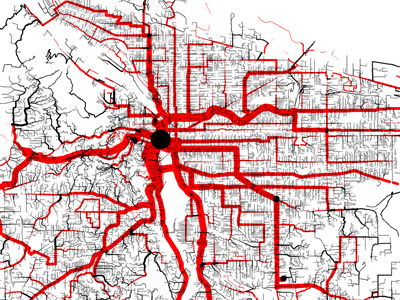
\includegraphics[width=0.4\linewidth]{img/shortest-path-tree}
\end{figure}
\end{frame}



\begin{frame}{Algoritmo de Dijkstra}
\framesubtitle{Pseudocódigo}

\begin{algorithm}[H]
	\DontPrintSemicolon
	
	$Q \gets V$\;
	Set $d(v) = \infty$ and $p(v) = -1$ for each $v \in V$\;
	$d(s) = 0$\;
	
	\While{$Q \neq \emptyset$}{
		$u \gets$ extract-min($Q$)\;
		\For{each $v$ adjacent to $u$}{
			\If{$d(v) > d(u) + w(u, v)$}{
				$d(v) \gets d(u) + w(u, v)$\;
				$p(v) \gets u$\;
			}
		}
	}
	
	\caption{\texttt{Dijkstra(Vertex s)}}
\end{algorithm}

\pause

\begin{itemize}
	\item Sempre que um elemento é extraído de $Q$, foi descoberto o menor caminho até ele (predecessor e custo).
	
	\item Quando todos os elementos foram removidos, todos os caminhos mínimos de $s$ a todos os demais vértices foram determinados.
\end{itemize}
\end{frame}



\begin{frame}{Algoritmo de Dijkstra}
\framesubtitle{Exercício de aplicação}

\begin{itemize}
	\item Considere o grafo apresentado abaixo. Simule a execução do algoritmo de Dijkstra para encontrar os caminhos mínimos de $A$ para todos os demais vértices.
\end{itemize}

\begin{figure}[width=0.5\textwidth]
	\begin{tikzpicture}[
		> = stealth,
		shorten > = 1pt,
		auto,
		node distance = 3cm,
		semithick,
		scale=0.7,
		transform shape
	]
	
	\tikzset{every state}=[
		draw = black,
		thick,
		fill = white,
		minimum size = 1mm
	]
	
	\node[state] (C) {$C$};
	\node[state] (D) [right=of y1] {$D$};
	\node[state] (A) [above=of y1]{$A$};
	\node[state] (B) [above=of y2] {$B$};
	
	\path[->] (A) edge  node[] {5} (B);
	\path[->] (A) edge  node[pos=0.25,below right] {1} (C);
	\path[->] (C) edge  node[pos=0.25,above right] {11} (D);
	\path[->] (B) edge  node[] {3} (D);
	\path[->] (A) edge  node[above] {9} (D);
	\end{tikzpicture}
\end{figure}
\end{frame}



\begin{frame}{Algoritmo de Dijkstra}
\framesubtitle{Detalhes}

\begin{itemize}
	\item \textbf{Complexidade:}
	\begin{itemize}
		\item O pré-processamento é executado em $O(n)$.
		\item O laço externo executa para cada vértice do grafo -- $O(n)$.
		\item A extração de $Q$ custa $O(\log n)$ usando um heap binário.
		\item O laço interno executa exatamente $m$ vezes (todos os arcos).
		\item Cada atualização de vértices implica em atualizar $Q$, o que custa $O(\log n)$.
		\item Complexidade total: $O(m \log n)$.
	\end{itemize}
	
	\medskip
	
	\item \textbf{Limitações:}
	\begin{itemize}
		\item O algoritmo não funciona com pesos negativos.
		\item Ineficiente para calcular o caminho simples entre um par de vértices.
	\end{itemize}
\end{itemize}
\end{frame}



\begin{frame}{Busca de caminho entre um par de vértices}

\begin{itemize}
	\item Algoritmo de Dijkstra gasta processamento para determinar todos os caminhos mínimos a partir de $s$.
	\item Caso apenas o caminho de $s$ a $t$ seja de interesse, podemos parar o algoritmo quando $t$ é removido de $Q$ e retornar o caminho encontrado.
	
	\item Existe forma mais eficiente?
	\begin{itemize}
		\item Sim, podemos guiar a busca em direção ao vértice de destino.
		\item \textbf{Algoritmo A*}!
	\end{itemize}

	\item O A* é o algoritmo mais utilizado para busca de caminhos em grafos.
	\item Veremos a aplicação do A* para grafos \textbf{não-ponderados}.
	\begin{itemize}
		\item A aplicação para grafos ponderados pode ser feita com ajustes simples.
	\end{itemize}
	\item Aplicações populares: jogos, inteligência artificial, roteamento. 
\end{itemize}
\end{frame}



\begin{frame}{Busca de caminho entre um par de vértices}
\framesubtitle{Dijkstra \textit{versus} A*}

\begin{columns}
	\begin{column}{0.5\textwidth}
		\begin{figure}
			\centering
			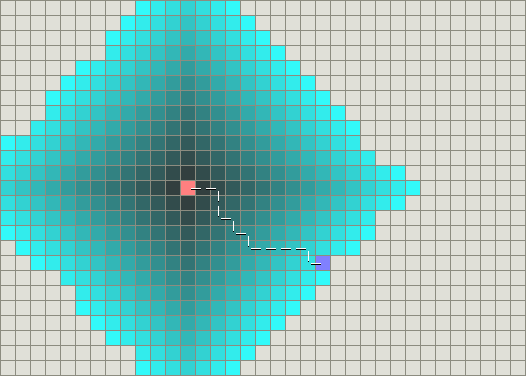
\includegraphics[width=\linewidth]{img/dijkstra}
		\end{figure}
	\end{column}
	\begin{column}{0.5\textwidth}
		\begin{figure}
			\centering
			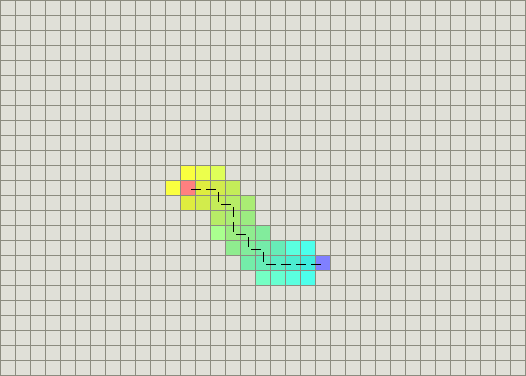
\includegraphics[width=\linewidth]{img/a-star}
		\end{figure}
	\end{column}
\end{columns}
\end{frame}



\begin{frame}{Busca A*}
\framesubtitle{Ideia geral}

\begin{itemize}
	\item A fila de prioridades usa uma função $f(v)$ para determinar a prioridade do vértice $v$.
	\item A função é composta por dois componentes: $f(v) = g(v) + h(v)$.
	\begin{itemize}
		\item $g(v)$ é a função de custo, dada pela distância $s$ a $v$.
		\item $h(v)$ é a função heurística, dada pela \textbf{estimativa de distância} de $v$ a $t$.
	\end{itemize}

	\item A busca é guiada pelo custo em se chegar ao vértice selecionado ($g(v)$), mas também o quão próximo ele está do objetivo ($h(v)$).
\end{itemize}
\end{frame}



\begin{frame}{Busca A*}
\framesubtitle{Pseudocódigo}

\begin{itemize}
	\item Dado um grafo não-ponderado, podemos escrever o algoritmo A* como:
\end{itemize}

\begin{algorithm}[H]
	\DontPrintSemicolon
	
	$Q \gets \{s\}$\;
	Set $p(v) = -1$ and $v$ not marked for each $v \in V$\;
	
	\While{$Q \neq \emptyset$}{
		$u \gets$ extract-min($Q$)\;
		\If{$u = t$}{
			\Return{path from $s$ to $t$}\;
		}
		
		\For{each $v$ adjacent to $u$}{
			\If{$v$ is not marked}{
				Set $v$ marked\;
				$p(v) \gets u$\;
				Add $v$ to $Q$\;
			}
		}
	}
	
	\caption{\texttt{A$^\texttt{*}$(Vertex s, Vertex t)}}
\end{algorithm}
\end{frame}



\begin{frame}[b]{Busca A*}
\framesubtitle{Função heurística}

\begin{itemize}
	\item Esta função estima a distância de um vértice até o vértice de destino.
	\item É sensível ao contexto, isto é, ao problema que está sendo resolvido.
	\pause
	\item \textbf{Exemplo:} dado um grafo que representa as cidades de um país, encontra o menor caminho desde uma cidade até outra.
\end{itemize}

\begin{figure}
	\centering
	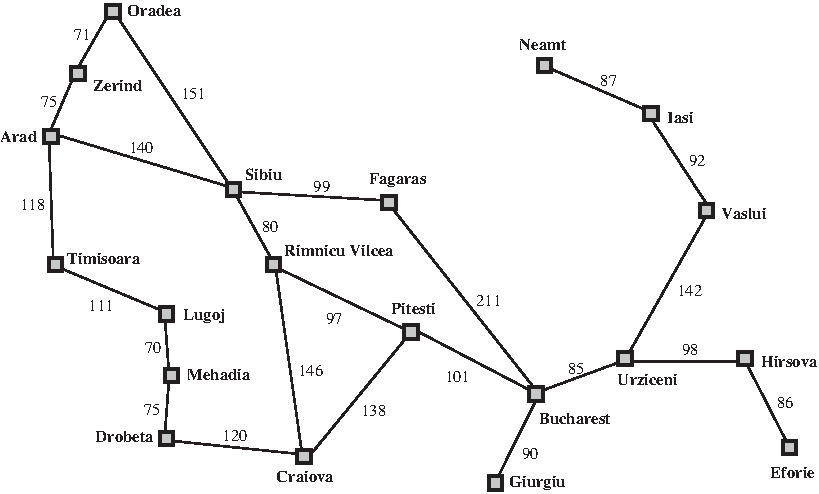
\includegraphics[width=0.7\linewidth]{img/grafo-cidades-roteamento}
\end{figure}
\end{frame}



\begin{frame}[b]{Busca A*}
\framesubtitle{Função heurística}

\begin{itemize}
	\only<1>{
		\item Consideremos a cidade de origem \textit{Sibiu}, com destino a \textit{Bucharest}.
		\item $g(v)$ é o custo de sair de \textit{Sibiu} até $v$.
		\item $h(v)$ é uma estimativa de distância de $v$ até \textit{Bucharest}.
	}

	\only<2>{
		\item Neste caso, $h(v)$ pode ser a distância em linha reta de $v$ até \textit{Bucharest}.
	}
\end{itemize}

\begin{figure}
	\centering
	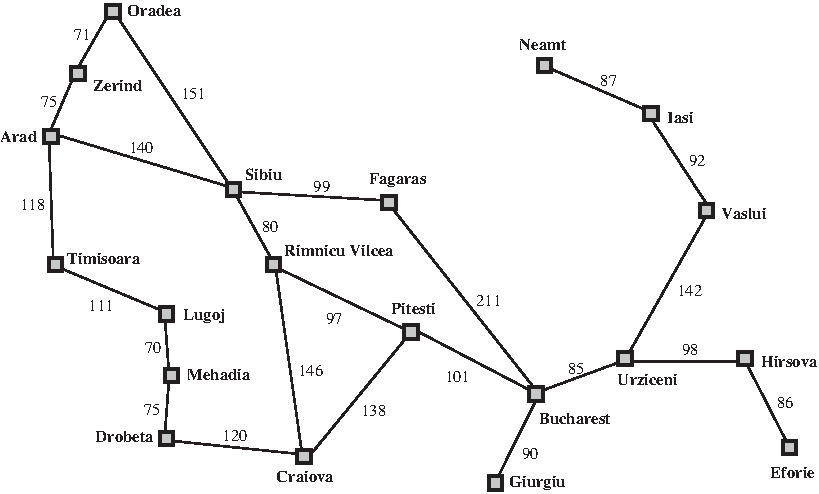
\includegraphics[width=0.7\linewidth]{img/grafo-cidades-roteamento}
\end{figure}
\end{frame}



\begin{frame}{Busca A*}
\framesubtitle{Otimalidade do algoritmo}

\begin{itemize}
	\item O algoritmo A* é ótimo, desde que a função heurística seja \textbf{admissível}.
	\item Uma função admissível é aquela que \textbf{nunca superestima} o custo para alcançar o objetivo.
	\begin{itemize}
		\item Ou seja, o custo estimado nunca é superior ao custo real.
	\end{itemize}
\end{itemize}
\end{frame}



\begin{frame}{Busca A*}
\framesubtitle{Exercício de aplicação}

\begin{itemize}
	\item Considere o grafo apresentado abaixo. O valor numérico nos vértices representa a função heurística para o mesmo. Simule a execução do algoritmo A* para encontrar o caminho mínimo de $A$ a $D$.
\end{itemize}

\begin{figure}[width=0.5\textwidth]
	\begin{tikzpicture}[
		> = stealth,
		shorten > = 1pt,
		auto,
		node distance = 3cm,
		semithick,
		scale=0.7,
		transform shape
	]
	
	\tikzset{every state}=[
		draw = black,
		thick,
		fill = white,
		minimum size = 1mm
	]
	
	\node[state] (C) {$C(8)$};
	\node[state] (D) [right=of y1] {$D(0)$};
	\node[state] (A) [above=of y1]{$A(6)$};
	\node[state] (B) [above=of y2] {$B(1)$};
	
	\path[->] (A) edge  node[] {5} (B);
	\path[->] (A) edge  node[pos=0.25,below right] {1} (C);
	\path[->] (C) edge  node[pos=0.25,above right] {11} (D);
	\path[->] (B) edge  node[] {3} (D);
	\path[->] (A) edge  node[above] {9} (D);
	\end{tikzpicture}
\end{figure}
\end{frame}


\begin{frame}{Outros algoritmos para caminhos}

\begin{itemize}
	\item Para árvores de caminhos mínimos em grafos não-ponderados:
	\begin{itemize}
		\item Busca em largura.
	\end{itemize}
	
	\item Para pesos negativos: 
	\begin{itemize}
		\item Bellman-Ford.
	\end{itemize}
	
	\item Para caminhos entre todo par de vértices: 
	\begin{itemize}
		\item Floyd-Warshall.
		\item Algoritmo de Johnson.
	\end{itemize}
	
\end{itemize}
\end{frame}



\begin{frame}{Exercício}
	\framesubtitle{Busca de caminhos}
	
	\begin{enumerate}
		\item Crie um programa que receba a descrição de um grafo dirigido e ponderado (vértices, arcos, pesos) e permita a busca de caminhos no grafo. O usuário poderá selecionar um vértice de origem $s$ e verificar o caminho mínimo de $s$ até todos os demais vértices. O usuário também poderá informar um par de vértices e checar o menor caminho entre eles. Para isso, implemente os algoritmos de busca de Dijkstra e A*.
	\end{enumerate}
\end{frame}


\frame{
	\frametitle{Referências}	
	\setlength{\bibsep}{8pt plus 0.3ex}
	\fontsize{10pt}{10}\selectfont
	\bibliographystyle{apalike}
	\bibliography{../referencias}
}

\end{document}